\documentclass[12pt]{standalone}

\usepackage{tikz}
\usepackage{ctex}

\begin{document}
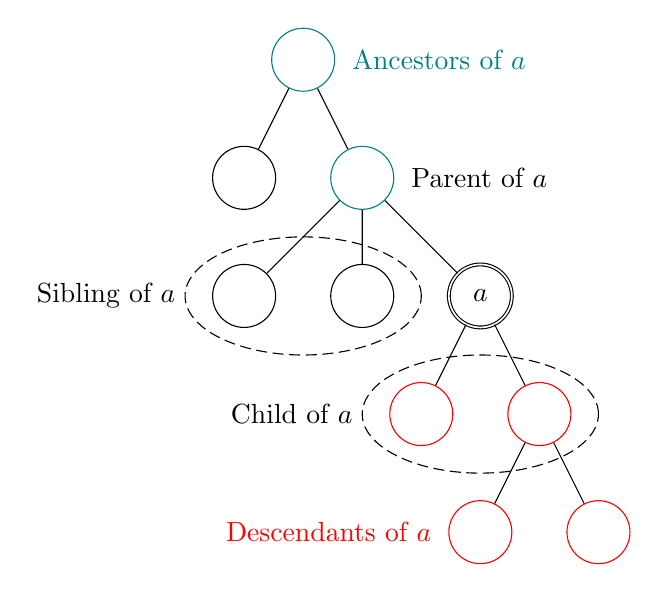
\begin{tikzpicture}

    \scoped[every node/.style={circle,draw,minimum size=8mm}]
    \node[draw=teal] (A) at (0,0) {}
        child {node (B) {}}
        child {node[draw=teal] (C) {}
            child {node (D) {}}
            child {node (E) {}}
            child {node[double] (F) {$a$}
                [every node/.style={circle,draw=red,minimum size=8mm}]
                child {node (G) {}}
                child {node (H) {}
                    child {node (I) {}
                        node[left=5mm,rectangle,draw=none,color=red] {Descendants of $a$}}
                    child {node (J) {}}}}
            node[right=5mm,rectangle,draw=none] {Parent of $a$}}
        node[right=5mm,rectangle,draw=none,text=teal] {Ancestors of $a$};

    \draw[dash pattern=on 4pt off 2pt] (0,-3cm)
        circle[x radius=1.5cm,y radius=0.75cm]
        node[left=1.5cm] {Sibling of $a$};

    \draw[dash pattern=on 4pt off 2pt] (2.25cm,-4.5cm)
        circle[x radius=1.5cm,y radius=0.75cm]
        node[left=1.5cm] {Child of $a$};

\end{tikzpicture}
\end{document}
